\documentclass[10pt]{article}

\addtolength{\oddsidemargin}{-.875in}
\addtolength{\evensidemargin}{-.875in}
\addtolength{\textwidth}{1.75in}

\addtolength{\topmargin}{-.875in}
\addtolength{\textheight}{1.75in}

\openup 1em

%macro for commenting
\usepackage{color}
\newcommand{\leo}[1]{{\color{blue}{LD: #1}}}

% \newcommand{\Xbeta}{ X_i \theta}
\newcommand{\xbeta}{ x_i \beta}
\newcommand{\xtheta}{ x_i \theta}
% \newcommand{\xbetaij}{ x_{ij}^T \theta}
\newcommand{\sgamma}{s_{ij}^T\gamma_i}

\usepackage[round]{natbib}

\usepackage{rotating}
\usepackage{graphicx}
\usepackage{subcaption}

\usepackage{float}
\usepackage{bbm}

\usepackage{amsthm,amsmath, amssymb} 
\usepackage{mathrsfs}
\usepackage{subcaption}
\usepackage{nicefrac}

\newtheorem{theorem}{Theorem}
\newtheorem{lemma}{Lemma}
\newtheorem{corollary}{Corollary}
\newtheorem{remark}{Remark}


\usepackage{algorithm}
\usepackage{algpseudocode}

%\usepackage{mhequ}
\newcommand{\be}{\begin{equation}\begin{aligned}}
\newcommand{\ee}{\end{aligned}\end{equation}}
\newcommand{\bb}[1]{\mathbb{#1}}
\newcommand{\mc}[1]{\mathcal{#1}}
\DeclareMathOperator{\Binom}{Binomial}
\DeclareMathOperator{\No}{No}
\DeclareMathOperator{\PG}{PG}
\DeclareMathOperator{\IG}{Inverse-Gamma}
\DeclareMathOperator{\Ga}{Gamma}
\DeclareMathOperator{\Bern}{Bernoulli}
\DeclareMathOperator{\U}{Uniform}
\DeclareMathOperator{\Poi}{Poisson}
\DeclareMathOperator{\NB}{NB}
\DeclareMathOperator{\cov}{cov}
\DeclareMathOperator{\var}{var}
\DeclareMathOperator{\diag}{diag}
\DeclareMathOperator{\Diag}{Diag}
\newcommand{\KL}[2]{\textnormal{KL}\left(#1 \parallel #2\right)}

\DeclareMathOperator{\1}{\mathbbm{1}}


\DeclareMathOperator{\bigO}{\mc O}



\thispagestyle{empty}
\baselineskip=28pt

\title{\textbf{Extrinsic Priors for Bayesian Modeling with Parameter Constraints}}
\author{Leo Duan, Akihiko Nishimura, David Dunson}
\date{}
\begin{document}
\maketitle
{\bf Abstract:} Prior information often takes for the form of parameter constraints. Bayesian methods include such information through prior distributions having constrained support. By using posterior sampling algorithms, one can quantify uncertainty without relying on asymptotic approximations. However, outside of narrow settings, parameter contraints make it difficult to develop efficient posterior sampling algorithms. We propose a general solution, which relaxes the constraint through the use of an {\em extrinsic prior}, which is concentrated close to the constrained space. General off the shelf posterior sampling algorithms, such as Hamiltonian Monte Carlo (HMC), can then be used directly. We illustrate this approach through multiple examples involving equality and inequality constraints. While existing methods tend to rely on conjugate families, our proposed approach frees us up to define new classes of hierarchical models for constrained problems. We illustrate this through application to a variety of simulated and real datasets.
\vskip 12pt
%\baselineskip=12pt
%\par\vfill\noindent
{\noindent KEY WORDS: Constraint relaxation; Euclidean Embedding; Monotone Dirichlet; Soft Constraint; Stiefel Manifold; Projected Markov chain}
%\par\medskip\noindent
%\clearpage\pagebreak\newpage
\pagenumbering{arabic}


\section{Introduction}
It is extremely common to have prior information available on parameter contraints in statistical models. For example, one may have prior knowledge that a vector of parameters lies on the probability simplex or satisfies a particular set of inequality constraints. Other common examples include shape constraints on functions, positive semidefiniteness of matrices and orthogonality. There is a very rich literature on optimization subject to parameter contraints. One common approach is to rely on Langrange and Karush-Kuhn-Tucker multipliers \citep{boyd2004convex}. However, simply producing a point estimate is often insufficient, as uncertainty quantification (UQ) is a key component of most statistical analyses. Usual large sample asymptotic theory, for example showing asymptotic normality of statistical estimators, tends to break down in constrained inference problems. Instead, limiting distributions may have a complex form that needs to be rederived for each new type of constraint, and may be intractable. An appealing alternative is to rely on Bayesian methods for UQ, including the constraint through a prior distribution having restricted support, and then applying Markov chain Monte Carlo (MCMC) to avoid the need for large sample approximations.

Conceptually MCMC can be applied in a broad class of constrained parameter problems without complications \cite{gelfand1992bayesian}. However, in practice, a primary difficulty is designing a Markov transition kernel that leads to an MCMC algorithm with sufficient computational efficiency to be practically useful. Common default transition kernels correspond to Gibbs sampling, random walk Metropolis-Hastings, and (more recently) Hamiltonian Monte Carlo (HMC). Gibbs sampling relies on alternately sampling from the full conditional posterior distributions for the different parameters, ideally in blocks to improve mixing. Gibbs requires the conditional distributions to be available in a form that is tractable to sample from directly, limiting consideration to specialized models. In constrained problems, block updating is typically either not possible or very inefficient (e.g. relying on rejection sampling with a high rejection probability), and one-at-a-time updating can lead to extremely slow mixing. Random walk algorithms provide an alternative, but each step of the random walk must maintain the parameter constraint. A common approach is to apply a normal random walk and simply reject proposals that violate the constraint, but this can have very high rejection rates even if using an adaptive approach that learns the covariance based on the history of the chain. An alternative is to rely on HMC. In simple settings in which a reparameterization can be applied to remove the constraint, HMC can be applied easily. Otherwise, HMC will generate proposals that violate the constraint, and hence face problems with high rejection rates in heavily constrained problems.

Due to the above hurdles, most of the focus in the literature has been on customized solutions developed for specific constraints.
One popular strategy is to carefully pick a prior and likelihood such that posterior sampling is tractable. For example, for modeling of data on manifolds, it is typical to restrict attention to specific models, such as the Bingham-von Mises-Fisher distribution for Stiefel manifolds \citep{khatri1977mises,hoff2009simulation}. For data on the probability simplex, one instead relies on the Dirichlet distribution. An alternative is to reparameterize the model to eliminate or simplify the constraint. For example, when faced with a monotonicity constraint, one may reparameterize in terms of differences as the resulting positivity constraint leads to much easier sampling (REFs). In the literature on modeling of data on manifolds, there are two strategies: (i) {\em intrinsic} methods that define a statistical model directly on the manifold, and (ii) {\em extrinsic} methods that indirectly induce a model on the manifold through embedding the manifold in a Euclidean space, defining a model in the Euclidean space, and then projecting back onto the manifold. Essentially all of the current strategies for Bayesian modeling with constraints take an intrinsic-style approach. However, by strictly maintaining the constraint at all stages of the modeling and computation process, one limits the possibilities in terms of defining general methods to deal with parameter constraints.

These drawbacks motivate the development of {\em extrinsic} approaches that define an unconstrained model and/or computational algorithm, and then somehow adjust for the constraint. A related idea is \cite{gelfand1992bayesian}, who suggested running Gibbs sampling ignoring the constraint but only accepting the draws satisfying the constraint. Unfortunately, such an approach is highly inefficient, as motivated above. An alternative is to run MCMC ignoring the constraint, and then project draws from the unconstrained posterior to the appropriately constrained space. Such an approach was proposed for generalized linear models with order constraints by \cite{dunson2003bayesian}, extended to functional data with monotone or unimodal constraints \cite{gunn2005transformation}, and recently modified to nonparametric regression with monotonicity \cite{lin2014monogp} or manifold \cite{lin2016extrinsic} constraints.

An alternative idea is to {\em relax} a sharp parameter constraint by defining a prior that has unrestricted support but places small probability outside of the constrained region. \cite{neal2011mcmc} suggested such an approach to apply HMC in settings involving a simple truncation constraint, while \cite{pakman2014exact} applied a related idea to improve sampling from truncated multivariate normal distributions.

The goal of this article is to dramatically generalize these specific approaches to develop a broad class of {\em extrinsic priors} for parameter constrained problems. These priors are defined to place small probability outside of the constrained region, while permitting use of efficient and general use MCMC algorithms; in particular, HMC. When the constraints need to upheld strictly, the approximation can be corrected with a simple projection, followed by a Metropolis-Hastings step with high acceptance probability.
Unlike intrinsic methods, such as Riemannian and geodesic HMC \citep{girolami2011riemann,byrne2013geodesic}, our approach is
relatively efficient and simple to implement in general settings using automatic algorithms. The generality frees up a much broader spectrum of Bayesian models, as one no longer needs to focus on very specific computationally tractable models.
Theoretic studies are conducted and original models are shown in simulations and data applications.

\section{Extrinsic Bayes Methodology}
\subsection{Intrinsic Bayes}
Let $\theta \in \mc D$ denote the parameters in likelihood function $L(\theta;y)$, with $y$ the data. The support $\mc D$ is a constrained space. The usual Bayesian approach assigns a prior density $\pi_{0,\mc D}(\theta)$ for $\theta$ having support $\mc D$. We assume that $\mc D \subset \mc R$, with $\mc R$ denoting a `less constrained' space. For example, if $\theta$ is a $p$-dimensional vector subject to an inequality constraint, then $\mc R$ may correspond simply to $p$-dimensional Euclidean space.
Assuming $\pi_{0,\mc D}(\theta)$ is proper so that $\int_{\mc D} \pi_{0,\mc D}(\theta) d\theta =1$, the constrained prior can be obtained by starting with an unconstrained prior $\pi_{0,\mc R}(\theta)$ on $\mc R$, applying the restriction through an indicator function $\mathbbm{1}_{\theta\in \mc D}$, and renormalizing:
\begin{equation}
\begin{aligned}
\label{exact_prior1}
\pi_{0,\mc D}(\theta)= \pi_{0,\mc R}(\theta \mid \theta \in \mc D) = \frac{ \pi_{0,\mc R}(\theta) \mathbbm{1}_{\theta\in \mc D} }{ \int_{\mc D} \pi_{0,\mc R}(\theta)d\theta },
\end{aligned}
\end{equation}
if $ \int_{\mc D} \pi_{0,\mc R}(\theta)d\theta >0$. When $ \int_{\mc D} \pi_{0,\mc R}(\theta)d\theta =0$, the construction becomes more complicated.

 One strategy to overcome the difficulty is using the regular conditional probability for certain set $\mc A$, via the limit
\begin{equation}
\begin{aligned}
\label{exact_prior2}
\int_{\mc A} \pi_{0,\mc D}(\theta) d\theta=\lim_{\mc D^+\supset \mc D} \frac{\int_{\mc A} \pi_{0,\mc R}(\theta) \mathbbm{1}_{\theta\in \mc D^+ } d\theta}{ \int_{\mc D^+} \pi_{0,\mc R}(\theta)d\theta }\end{aligned}
\end{equation}
where $\mc D^+$ is a net converging towards $\mc D$, with $\int_{\mc D^+} \pi_{0,\mc R}(\theta)d\theta>0$. Based on this probability, one derives the constrained density. To illustrate, consider two independent uniform distribution $\theta_1,\theta_2 \sim \U(0,1)$ under equality constraint $\theta_1+\theta_2=w$. One first obtains $\int_{\theta_1<x}\pi_{0,\mc D}(\theta) d\theta=\lim_{\epsilon\rightarrow 0^+} \frac{ \int_0^{x} \int_0^1 \mathbbm{1}_{\theta\in \mc D^+}  d\theta_2d\theta_1} { \int_0^1 \int_0^1 \mathbbm{1}_{\theta\in \mc D^+}  d\theta_2d\theta_1 } =\frac{x}{w}$ with $\mc D^+= \{ \theta: \theta_1+\theta_2\in (w-\epsilon, w+\epsilon)\}$, and then obtained constrained density $\pi_{0,\mc D}(\theta_1)= \frac{1}{w}$ with $\theta_2=w-\theta_1$.

\subsection{Extrinsic Prior}
Our extrinsic prior builds on the intrinsic prior in \eqref{exact_prior1} and \eqref{exact_prior2}, approximating the sharp indicator function
$\mathbbm{1}_{\theta\in \mc D}$ with a {\em smooth} alternative having less constrained support.

\begin{equation}
\label{extrinsic_prior}
	\tilde{\pi}_{0,\mc D}(\theta) = \frac{ \pi_{0,\mc R}(\theta) \mc{K}( \theta; \mc D) }{ \int_{\mc R} \pi_{0,\mc R}(\theta) \mc{K}(\theta; \mc D)d\theta }
\end{equation}
where $\mc K(\theta; \mc D)$ is an approximation to $\mathbbm{1}_{\theta\in \mc D}$ and satisfies  $ \int_{\mc R} \pi_{0,\mc R}(\theta) \mc{K}(\theta; \mc D)d\theta>0$.

Let the constraints that define $\mc D$ be broken into $m$ separable parts, with each corresponding to a constrained space $\mc D_k$. We have $\mc D = \bigcap_{k=1}^m\mc D_k$ and define $\mc K$ as:
\begin{equation}
\label{smoothing}
\mc K(\theta; \mc D)= \prod_{k=1}^m K_k(v_k(\theta))
\end{equation}
where $v_k$ is a function $v_k: \mc R \rightarrow [0,\infty)$ that measures the ``distance'' to the space $\mc D_k$, with $v_k(\theta)=0$ when $\theta\in \mc D_k$; $K_k(v_k(\theta))$ is a function $K_k:[0,\infty)\rightarrow [0,1]$, which decreases in $v_k(\theta)$, with $K_k(0)=1$ and $K_k(\infty)=0$. Therefore,  $\theta\in \mc D$ and $\mc K(\theta;\mc D)=1$ if and only if all $v_k(\theta)=0$. In this paper, we focus on a simple exponential function $K_k(v(\theta)) = \exp(-v(\theta)/\lambda_k)$, with $\lambda_k>0$ as the tuning parameter.

The distance function $v(\theta)$ is often easy to find. For example, a large class of models can be viewed as constrained under  equality $f(\theta)=0$ and/or inequality $f(\theta)<0$ . The distance to equality constraint can be $v(\theta)=|f(\theta)|$; the distance to inequality can be $v(\theta)=|f(\theta)|_+$, where $(x)_+ = \left\{\begin{array}{cc}  0 \text{ if } x\le 0 \\ x \text{ if } x> 0\end{array}\right.$. More complicated constraint can be defined similarly. For example, for $\theta\in \mathbb{R}^{n\times p}$ with orthonormality constraint $\theta'\theta=I_p$, the distance can be $v(\theta) = ||\theta'\theta-I_p||_{k}$ with $||x||_k=(\sum_{ij} |x_{ij}|^k)^{1/k}$.


To illustrate the extrinsic prior, consider a truncated normal prior $\No_{(-\infty,5)}(0,5^2)$. Figure~\ref{truncated_normal} plots the unnormalized densities of intrinsic prior $\pi_{0,\mc R}\mathbbm{1}_{\theta\in \mc D}=\exp(-{\theta^2}/{2\cdot 5^2})\mathbbm{1}_{\theta\in (-\infty,5)}$ and extrinsic priors $ \pi_{0,\mc R}(\theta) \mc{K}( \theta; \mc D) = \exp(-{\theta^2}/{2\cdot 5^2}) \exp(-v(\theta))$. For the latter, we consider $2$ distances $v(\theta)$: $(\theta-5)_+$, $(\theta-5)^2_+$. Inside $\mc D$, The intrinsic and extrinsic priors are the same up to a constant difference due to normalizing. Outside $\mc D$, the extrinsic prior decreases continuously towards 0, while intrinsic prior discontinuously drops to $0$ at the boundary. With the same $\lambda$, first-order distance $(\theta-5)_+$ drops faster than second-order $(\theta-5)_+^2$ when $(\theta-5)_+<1$. %In general, one would prefer $v(\theta)$ to be small with most less than $1$, therefore, first-order $v(\theta)$ is commonly preferrable.

\begin{figure}[H]
 \centering
 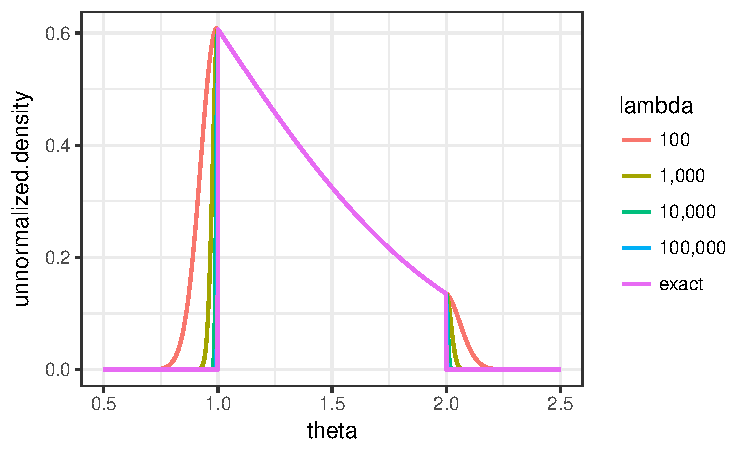
\includegraphics[width=0.5\textwidth]{density_truncated_normal}
\caption{Unnormalized densities for truncated normal $\No_{(-\infty,5)}(0,5^2)$ under exact intrinsic prior and approximating extrinsic prior. Inside $(-\infty,5)$, the priors are the same up to a constant difference. The intrinsic prior abruptly drops to $0$ on the boundary, while the approximating ones drop continuously. Intrinsic prior based on first-order $v(\theta)$ drops faster than the one based on second order when $v(\theta)\in (0,1)$.}
\label{truncated_normal}
\end{figure}


This smoothing function $\mc K(\theta;\mc D)$ in \eqref{smoothing} is applicable to more general and complicated scenarios. For example, $\theta$ can have some parameters constrained and some unconstrained; some parameters can be in multiple constraints simultaneously; constraints can be dependent. In all these cases, one can find proper $\mc D_k$'s and define $v_k(\theta)$'s accordingly.

\subsection{Property of Extrinsic Prior}

We now study the properties of the extrinsic prior. One important task is to quantify the difference between extrinsic and intrinsic priors. We first focus on the first case in \eqref{exact_prior1}, when $\int_{\mc D} \pi_{0,\mc R}(\theta)d\theta>0$.

%distance between extrinsic and intrinsic
\begin{remark}
Let $M_1= \int_{\mc D} \pi_{0,\mc R}(\theta)d\theta$ and $M_2 = \int_{\mc R} \pi_{0,\mc R}(\theta) \mc K(\theta;\mc D)d\theta$, when $M_1>0$, the total variation distance between the measures of extrinsic and intrinsic prior
$$||\pi_{0,\mc D}(\theta), \tilde{\pi}_{0,\mc D}(\theta) ||_{TV} = 1 - \frac{M_1}{M_2} \le \frac{\int_{\theta  \in \mc R \setminus \mc D} \pi_{0,\mc R}(\theta) \mc K(\theta;\mc D)d\theta}{M_1}$$.
\end{remark}
proof:
{via definition of total variation distance and $K(\theta;\mc D)=1$ when $\theta\in\mc D$, $0$ otherwise.}


In the case of exponential smoothing function \eqref{smoothing}, we have:
\begin{corollary}
Let $M_1= \int_{\mc D} \pi_{0,\mc R}(\theta)d\theta>0$ and $\mc K(\theta; D) = \prod_{k=1}^m \exp( -v_k(\theta)/\lambda_k)$, one sufficient condition to have
$$\lim_{\text{ all } \lambda_k\rightarrow 0}||\pi_{0,\mc D}(\theta), \tilde{\pi}_{0,\mc D}(\theta) ||_{TV} = 0$$
is that $\pi_{0,\mc R}(\theta)$ is proper, $\int_{\mc R} \pi_{0,\mc R}(\theta) d\theta<\infty$.
\end{corollary}
proof:
{via dominated convergence theorem}

Rewriting $\mc K(\theta; D) = \exp(-v(\theta)/\lambda)$ with $\lambda = \sup_k \lambda_k$, $v(\theta)=\lambda\sum_{k=1}^m\frac{ v_k(\theta)}{\lambda_k}$, we obtain the convergence rate:

\begin{remark}
Assuming $M_3= \int_{\mc R \setminus \mc D} \pi_{0,\mc R}(\theta) d\theta<\infty$, and $f(v)$ be the density of $v(\theta)$ as the transform of $\pi_{0,\mc R}(\theta)/M_3$. If there exists an $t<\infty$ such that $f(v) < \infty$ for $v<t$,
$$\int_0^\infty {\pi_{0,\mc R}(\theta)}exp(- \frac{v(\theta)}{\lambda}) d \theta \le 
2 {M_3} \exp(-\frac{t}{\lambda}) + {M_3} \sup_{t^*\in(0,t)} {f(t^*)}\lambda 
$$
\end{remark}
proof:

\begin{equation}
\begin{aligned}
\int_0^\infty {f(v)} \exp(- \frac{v}{\lambda}) d v
= & \int_0^t {f(v)} \exp(- \frac{v}{\lambda}) d v + \int_t^\infty {f(v)} \exp(- \frac{v}{\lambda}) d v \\
% \le &  t\frac{f(t^*)}{M_3} \exp(- \frac{t^*}{\lambda})+ \exp(- \frac{t}{\lambda})  \int_t^\infty \frac{f(v)}{M_3} d v \\
% \le &  t\frac{f(t^*)}{M_3} \exp(- \frac{t^*}{\lambda})+ \exp(- \frac{t}{\lambda})\\
\le & {F(t)} \exp(-\frac{t}{\lambda}) + 
\frac{1}{\lambda}\int_0^t {F(v)} \exp(-\frac{v}{\lambda})dv + \exp(-\frac{t}{\lambda}) \\
= & ({F(t)} +1) \exp(-\frac{t}{\lambda}) + 
\frac{1}{\lambda}\int_0^t {f(v^*)} v\exp(-\frac{v}{\lambda})dv \\
\le & ({F(t)} +1) \exp(-\frac{t}{\lambda}) + \sup_{t^*\in(0,t)} {f(t^*)}
\int_0^t  \frac{1}{\lambda}v\exp(-\frac{v}{\lambda})dv \\
\le & 2 \exp(-\frac{t}{\lambda}) + \sup_{t^*\in(0,t)} {f(t^*)}\lambda 
\end{aligned}
\end{equation}
where $F(t)=\int_0^t f(x)dx$ and the third step is based on mean value theorem with $v^*\in (0,v)$. Rearranging term yields the result.  $\blacksquare$

That is, for $\lambda$ small, the extrinsic prior approaches intrinsic prior in total varation distance in $O(\lambda)$. The rate is quantified under very general assumption. We expect it can be sharpened under special cases.

We now examine the second case in \eqref{exact_prior2} where ${ \int_{\mc D} \pi_{0,\mc R}(\theta)d\theta }=0$.


\leo{this needs some more work}
\begin{remark}
Let $M_1(\mc D^+)= \int_{\mc D^+} \pi_{0,\mc R}(\theta)d\theta$ and $M_2 = \int_{\mc R} \pi_{0,\mc R}(\theta) \mc K(\theta;\mc D)d\theta$, with $\mc D^+$ chosen such that $M_1(\mc D^+)>0$ and $M_1(\mc D^+)<M_2$, the total variation distance between the measures of extrinsic and intrinsic prior

$$||\pi_{0,\mc D}(\theta), \tilde{\pi}_{0,\mc D}      (\theta) ||_{TV} = 1 - \frac{\lim_{\mc D^+\supset \mc D}\int_{\theta  \in \mc D^+} \pi_{0,\mc R}(\theta) \mc K(\theta;\mc D)d\theta}{M_2} = \frac{\lim_{\mc D^+\supset \mc D}\int_{\theta  \in \mc R \setminus \mc D^+} \pi_{0,\mc R}(\theta) \mc K(\theta;\mc D)d\theta}{M_2}$$.
\end{remark}

\section{Posterior Computation}

Letting the likelihood function be $L(y;\theta)$, the posterior distribution of $\theta$ under a extrinsic prior is
\begin{equation}
\label{extrinsic_posterior}
	\tilde{\pi}_{\mc D}(\theta \mid y) = \frac{ L(y;\theta)\pi_{0,\mc R}(\theta) \mc{K}( \theta; \mc D) }{ \int_{\mc R} L(y;\theta)\pi_{0,\mc R}(\theta) \mc{K}(\theta; \mc D)d\theta },
\end{equation}
which we refer as extrinsic posterior from now on. As it is supported on a less restrictive space $\mc R$, one can exploit conventional sampling approach such as slice sampling, adaptive Metropolis-Hastings and Hamiltonian Monte Carlo (HMC) for posterior sampling. In this section, we focus on HMC for its easiness to use and good performance in sampling with high-dimensional parameter.

\subsection{Hamiltonian Monte Carlo for Extrinsic Posterior Sampling}

We first provide a short review of Hamiltonian Monte Carlo for continuous $\theta$, although discrete extension is possible \citep{zhang2012continuous,nishimura2017discontinuous}.

Assuming $\theta\in\mc R$, with $\mc R$ in a full or truncated Eucledean space $\mathbb R^d$. HMC augments a latent variable ``momentum'' $p\in \mathbb R^d$ (commonly generated from $\No(0, \Sigma)$ with $\Sigma$ pre-specified), ommiting constant, the negative log-posterior function based on \eqref{extrinsic_prior} is

% To be clear, this is different from Riemannian HMC that requires specific accommodation and heavy computation. The algorithm we use is simply conventional HMC in Euclidean space. In this section, we study the effects of choosing $\lambda$ on efficiency of Hamiltonian dynamics.

\begin{equation}
\begin{aligned}
H(\theta, p)& = U(\theta)+M(p),\\
\text{where } & U(\theta) = -\log\left\{ L(\theta;y)\pi_{0,\mc R}(\theta) \mc{K}(\theta;\mc D) \right\},\\
& M(p) = \frac{p'\Sigma^{-1} p}{2},\end{aligned}
\end{equation}
Denoting current state as $(\theta^{(0)},p^{(0)})$, HMC updates $\theta$ and $p$ via Hamiltonian dynamics, defined by two partial differential equations:

\begin{equation}
\begin{aligned}
\label{hamiltonian}
\frac{\partial \theta (t)}{\partial t} & =\frac{\partial H(\theta, p)}{\partial p} = \Sigma^{-1}p,\\
\frac{\partial p(t)}{\partial t}& =-\frac{\partial H(\theta, p)}{\partial \theta} = -\frac{\partial U(\theta)}{\partial \theta}.
\end{aligned}
\end{equation}

By evolving in $t>0$, this yields $(\theta^{(t)},p^{(t)})$. Since Hamiltonian system is symplectic, i.e. $H(\theta^{(t)},p^{(t)})=H(\theta^{(0)},p^{(0)})$, one can take $\theta^{(t)}$ as a new posterior sample. However, in most cases, \eqref{hamiltonian} lacks closed-form solution, one has to use an {\it integrator} that numerically approximates an evolution of the exact solution. With the integrator reversible and volume-preserving (see \citep{neal2011mcmc} for details), an Metropolis-Hastings (M-H) step is taken to correct the approximation error, by accepting $(\theta^{(t)},p^{(t)})$ with probability 
$$1\wedge \exp  \left( - H(\theta^{(t)},p^{(t)}) + H(\theta^{(0)},p^{(0)}))\right)$$

One common integrator is the leap-frog algorithm \citep{neal2011mcmc}that utilizes move $(\theta^{(T\epsilon)}, p^{(T\epsilon)}) \rightarrow (\theta^{((T+1)\epsilon)}, p^{((T+1)\epsilon)})$:

\begin{equation}
\begin{aligned}
\label{leap-frog}
p \leftarrow p - \frac{\epsilon}{2} \frac{\partial U}{\partial  \theta },\quad
 \theta \leftarrow  \theta  + \epsilon \Sigma^{-1}p,\quad
p \leftarrow p -  \frac{\epsilon}{2}  \frac{\partial U}{\partial  \theta } 
\end{aligned}
\end{equation}
for $T=0,\ldots,(L-1)$; where $L$ is the number of leap-frog steps within one iteration and $t=L\epsilon$.


\subsection{Optimizing Computing Efficiency}

As a Markov chain Monte Carlo, one would hope to use HMC to build a chain that rapidly converges. The convergence rate is associated with the maximal correlation  \citep{liu2008monte}, $\gamma (\theta,\theta^*) = \sup_{g \in L^2(\Pi)} \mbox{corr}(g(\theta), g(\theta^*))
$, where $L^2(\Pi)=\{g(\theta): \mbox{var}(g(\theta))<\infty\}$. Smaller $\gamma (\theta,\theta^*)$ corresponds to less correlation and faster convergence. At fixed $\epsilon$, one can adaptively choosing $L$ so that $\gamma (\theta,\theta^*)$ falls under certain desired rate \citep{hoffman2014no}.

We now further examine this via a view of computing efficiency. Since each iterator step is often the bottleneck, one would use as few steps as possible to reach below the desired convergence rate.  Given a desired convergence rate $\gamma^*$, an optimal $\epsilon$ would be:

$$\epsilon^* =  \underset{\epsilon: \epsilon \le \epsilon_{max}}{\arg\inf}\inf_{L}\{L: \gamma \left(\theta^{(0)}, \theta^{(\epsilon L)} \right) \le \gamma^*   \},$$
where $\epsilon_{max}$ is the stability bound for the integrator step size. Given fixed integrator time $\epsilon L$, to minimize $L$, often the optimality occurs when $\epsilon\approx \epsilon_{max}$.

The stability bound $\epsilon_{max}$ can be influenced by the specification in extrinsic prior. The stability bound is roughly determined by the width of support in the most constrained direction  \citep{neal2011mcmc}. Formally, letting $\mc S_{\epsilon}$ be the contour region of the support $\mc S_{\epsilon}=\{x: \pi(x)\in (0,\epsilon)\}$ with $\pi(x)$ as the density, the minimum support width is:

$$w_\pi = \underset{{x_1\in \mc S_\epsilon}}{\inf}\underset{x_2\in \mc S_\epsilon}{\sup} \{ d(x_1, x_2): \pi(\alpha x_1 + (1-\alpha)x_2)>0 \text{ for } \alpha \in [0,1]  \}$$
where $d(.,.)$ is a metric, and is Eucledean distance in continous HMC.


To provide an intuition for why $\epsilon_{max}$ depends on $w_\pi$, we focus on one-step update $L=1$. Each update in leap-frog algorithm corresponds to $\theta^{(\epsilon)}=\theta^{(0)} + \epsilon  p^{(0)} - \epsilon^2/2  \frac{\partial U}{\partial  \theta } = \theta^{(0)} + \varepsilon  p^{(0)} + O(\epsilon^2)$. If $\epsilon \gg w_\pi$, a random move in $\varepsilon  p(0)$ can end outside the support with $U(\theta^{(\epsilon)})=\infty$. This would violate the condition that discrete integrator approximately preserves $U(\theta^{(\varepsilon)})+M(p^{(\varepsilon)}) = U(\theta^{(0)})+M(p^{(0)})< \infty$.

Therefore to efficiently utilize HMC, if the constrained space $\mc D$ has narrow support via certain direction in its embedded space $\mc R$, one needs to create more relaxation in extrinsic prior. For example, one equality constraint $x+y+z=1$ in $\mathbb{R}^3$ creates a hyperplane. Extrinsic prior with $\exp(- \frac{|x+y+z-1|}{\lambda})$ relaxes the support along the normal vector of the plane, creating a slab with some thickness greater than $0$. To have decent $\epsilon_{max}$, one needs to avoid choosing $\lambda$ too small. Empirically, we found $\lambda= 10^{-3}$ is often a good value for such constraint.


\section{Examples and Application}

We now use examples to illustrate the properties of extrisinc priors and their utility in complex real data application.

\subsection{Simulations}

{\bf Example 1: Unit Circle}

When the constrained support in $\mc D$ has small minimum support width $w_\pi$, it limits the stability bound. Therefore it is important to allow some support expansion to the corresponding constraint. We first illustrate such case via estimation on a unit circle. The circle has $w_\pi =0$ and therefore needs some support expansion to run HMC. 


Consider data $y_i\in \mathbb{R}^2$ for $i=1,\ldots,n$  that are noisy realization from one point on unit circle:

$$y_i\sim \No(\theta, I_2\sigma^2),\text{ with } \theta'\theta=1,$$
where $\theta \in \mc V(2,1)$, a $(2,1)$--Stiefel manifold, is assigned a von Mises--Fisher prior $\pi_{0,\mc D}(\theta) \propto \exp(F'\theta_i)$.

 To generate data, we use $\theta= (\sqrt 3/2, 1/2)$, $\sigma^2=0.5^2$ and small $n=5$, in order to induce widely spread-out posterior $\theta$ on the manifold. For posterior sampling, we use $F=(1,1)$ to induce a weakly informative prior for $\theta$ and an inverse-Gamma prior $\text{IG}(2,1)$ for $\sigma^2$ . To allow extrinsic posterior sampling, we use $v(\theta)=|\theta'\theta -1|$ as the distance to constrained space and extrinsic prior $\tilde\pi_{0,\mc D}(\theta)= \exp(F'\theta_i) \exp(-\frac{|\theta'\theta -1|}{\lambda})$.

We test three different tuning parameters  $\lambda = 0.001$, $0.0001$ and $0.00001$. We run each algorithm for $20,000$ steps, with first $10,000$ discarded. To compare the computing efficiency, we restrict the maximum leap-frog steps $L$ to be $100$ and visualize how much space each algorithm can explore within one HMC iteration. Figure~\ref{unit_circle}(a) plots the path of $L=100$ leap-frog steps. Larger $\lambda$ leads to wider support expansion and larger stability bound $\epsilon_{max}$. This makes $\theta^{(\epsilon L)}$  much less correlated with $\theta^{(0)}$ at each iteration, measured by autocorrelation (ACF) based on the posterior sample of $\theta_1$ (Figure~\ref{unit_circle}(b)). The posterior distribution of the distance $v(\theta)$ is small for all three settings (Figure~\ref{unit_circle}(c)), with smaller $\lambda$ associated with smaller $v(\theta)$

\begin{figure}[H]
\centering
   \begin{subfigure}[b]{0.8\textwidth}
    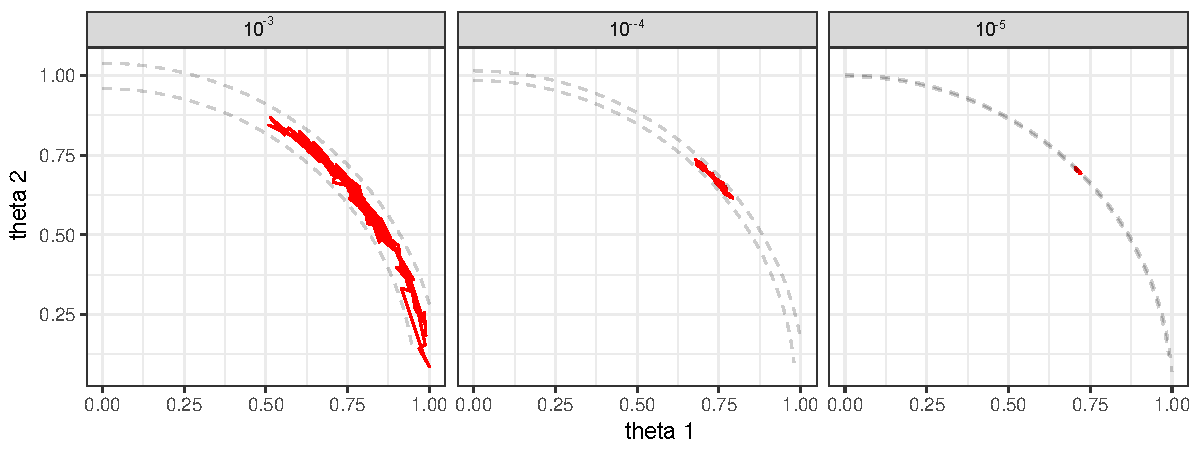
\includegraphics[width=1\textwidth]{unit_circle_100steps}
    \caption{Path of 100 itegrator steps in one HMC iteraton}
	\end{subfigure}
    \begin{subfigure}[b]{0.8\textwidth}
     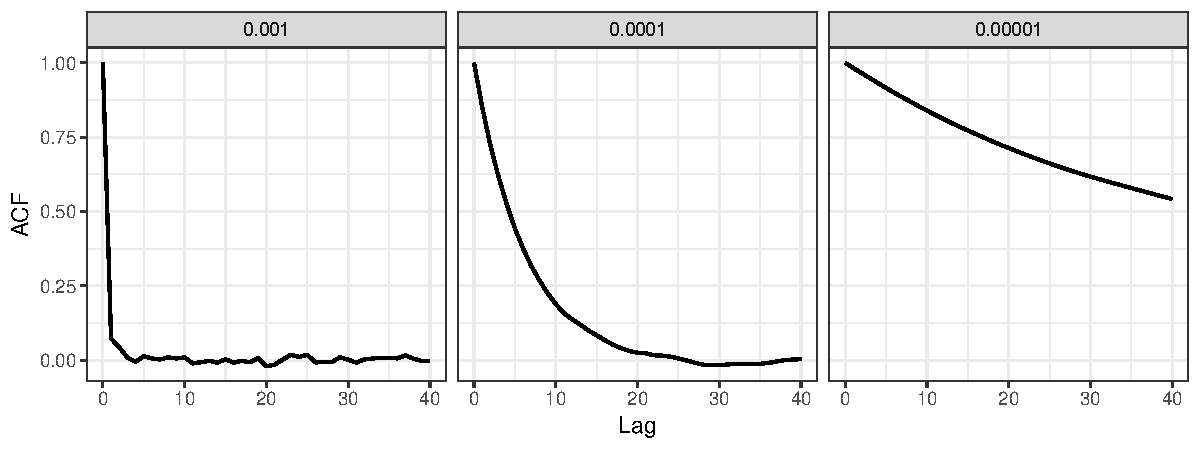
\includegraphics[width=1\textwidth]{unit_circle_acf}
     \caption{Autocorrelation of $\theta_1$}
     	\end{subfigure}
    \begin{subfigure}[b]{0.8\textwidth}
    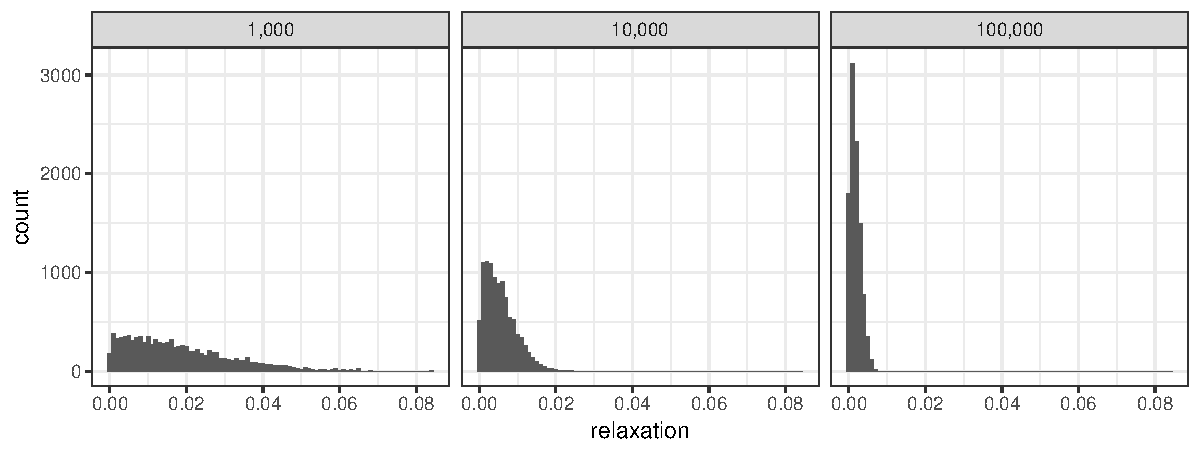
\includegraphics[width=1\textwidth]{unit_circle_violation}
         \caption{Posterior distribution of  $|\theta'\theta-1|$}
    	\end{subfigure}
\caption{HMC Sampling on a unit circle, using extrinc prior with $\mc K(\theta)=\exp(-\frac{|\theta'\theta -1|}{\lambda})$, with $\lambda=0.001$, $0.0001$ and $0.00001$. Panel (a) shows the larger relaxation in the narrowest direction of support (orthogonal vector to the circle) can result in more efficient space exploration within $100$ leap-frog steps; panel (b) shows the autocorrelation of the posterior sample; panel (c) shows the posterior distribution of the distance to the constraint.}
\label{unit_circle}
\end{figure}

{\bf Example 2: Linear Regression Under Inequality Constraint}

If the support on constrained space $\mc D$ does not have small minimum support width $w_\pi$, one can use extrinsic prior with almost no relaxation. This applies a large class of inequality constraints that has wide support. To illustrate, consider a linear regression

$$y_i \sim \No (x_i \theta, \sigma^2) \text{ for } i=1,\ldots n, \quad\text{ with } A\theta \le c$$
where both $\theta$ is a $p$-dimensional vector; $d$ many linear equalities are defined by $d\times p$ matrix  $A$ and a $d$-dimensional vector $c$. The inequalities form one or multiple polyhedrons in $\mathbb R^p$, with $\mc D$ as the interior or exterior space.

We consider simple bivariate case $\theta \in (0,1)^2$ subject to $\theta_1+\theta_2\le 1$, making $\mc D$ a triangle. To simulate data, we use $\sigma^2=0.1^2$, $x_i\sim \No([0,0]',I)$ for $i=1,\ldots,n$. We then generate two datasets with two different sets of $(\theta,n)$. In the first set, we use $\theta=[0.3,0.3]'$ with $n=10$, so that the posterior has wide spread in the constrained space; in the second set, we use $\theta=[0.7,0.3]'$ with $n=10^4$ so that the posterior is concentrated near the boundary. In both cases, we assign weakly informative prior for $\theta\sim \No([0.5, 0.5]',I10^2)$ and $\sigma^2\sim IG(2,1)$.

Unlike the unit circle example, the constrained space $\mc D$ has large $w_\pi$. This allows us to choose $\lambda=10^{-8}$ for $\mc K(\theta)=\exp( - \frac{|\theta_1+\theta_2-1|}{\lambda})$ in the extrinsic prior, leading to almost no constraint relaxation. We collect $10,000$ posterior samples efficiently via HMC. Figure~\ref{linear_inequality} plots the posterior sample and its contour. There is no posterior outside $\mc D$ due to the small $\lambda$.

\begin{figure}[H]
   \begin{subfigure}[b]{0.45\textwidth}
    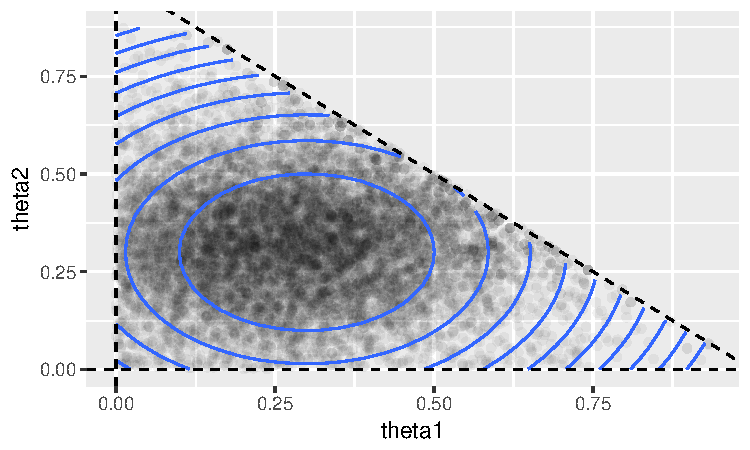
\includegraphics[width=1\textwidth]{linear_inequal_1}
    \caption{$n=10$ with true $\theta=[0.3,0.3]'$}
	\end{subfigure}
    \begin{subfigure}[b]{0.45\textwidth}
     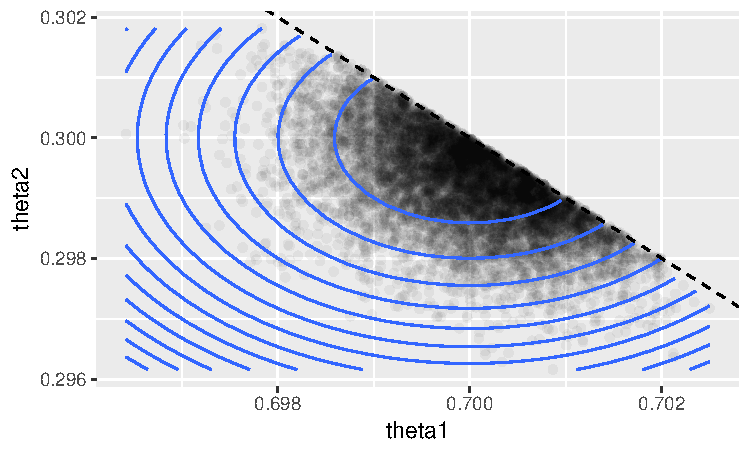
\includegraphics[width=1\textwidth]{linear_inequal_2}
     \caption{$n=10^4$ with true $\theta=[0.7,0.3]'$}
     	\end{subfigure}
\caption{Extrinsic posterior distribution of the normal mean $\theta$, with approximation to constraint $\theta_1+\theta_2\le 1$. Posterior is either loosely distributed near the center (panel (a)) or concentrated on the boundary (panel (b)) of the region. The extrinsic posterior has no samples outside of the region due to almost no relaxation.}
\label{linear_inequality}
\end{figure}

\subsection{Applications}

We now illustrate the utilitiy of extrinsic prior in two applications. 

{\bf Application 1: Ordered Dirichlet Prior}

We first use ordered simplex in finite mixture model. A $(J-1)$--simplex is a vector $w=\{w_1,\ldots w_J\}$ with $1> w_1 \ge \ldots \ge w_J > 0$ and $\sum_{j=1}^J w_j=1$.

For probablity simplex, standard practice assigns Dirichlet prior $Dir(\alpha)$, with $
\pi_{0, \mc D}(w) = \prod_{j=1}^J w_j^{\alpha-1} \1_{\sum_{j=1}^J w_j=1}$. However, this does not accomodate ordering; therefore, the index $j$ is exchangeable and permutating $j$'s does not change the density. This commonly leads to label-switching problem in mixture model estimation (reviewed in \cite{jasra2005markov}).

Imposing order constraint yields an ordered Dirichlet prior:

 \begin{equation}
\begin{aligned}
\label{ordered_dp_prior}
\pi_{0, \mc D}(w_1,\ldots w_J) = \prod_{j=1}^J w_j^{\alpha-1} \cdot \1_{\sum_{j=1}^J w_j=1} \cdot  \prod_{j=1}^{J-1}\1_{w_j \ge w_{j+1}}.
\end{aligned}
\end{equation}
where $w_j\in (0,1)$ for $j=1,\ldots,J$. The ordered Dirichlet prior can be approximated by extrinsic prior:


 \begin{equation*}
\begin{aligned}
\tilde\pi_{0, \mc D}(w_1,\ldots w_J) = \prod_{j=1}^J w_j^{\alpha-1} \cdot  \exp ( -  \frac{ \sum_{j=1}^J ( w_{j+1} - w_j )_+}{\lambda_1})
 \exp ( -  \frac{|{\sum_{j=1}^J w_j - 1}|}{\lambda_2})
\end{aligned}
\end{equation*}

We now adopt this simplex distribution in a normal mixture model with mixture means and common variance, for data $y_i\in \bb R^d$ indexed by $i=1,\ldots,n$:

\begin{equation*}
\begin{aligned}
y_i &\stackrel{indep}{\sim} \No(\mu_i,\Sigma),\qquad
\mu_i &\stackrel{iid}{\sim} G,\qquad
G(.) & = \sum_{j=1}^{J} w_j \delta_{\mu_j}(.),
\end{aligned}
\end{equation*}
where $\delta_{b}(a)=1$ if $a=b$ and $0$ otherwise.

We generate $n=100$ samples from $3$ components with true $\{w_1,w_2,w_3\}=\{0.6,0.3,0.1\}$ and two-dimensional means $\{\mu_1,\mu_2,\mu_3\} = \{[1,5], [3,3], [3,5]\}$ with identity covariance $\Sigma = I_2$. We assign weakly informative priors $\No(0,10 I_2)$ for each $\mu_j$ and inverse Gamma prior for the digonal element in $\Sigma=\diag(\sigma_1^2,\sigma_2^2)$ with $\sigma^2_1, \sigma^2_2\sim IG(2,1)$. We use $\lambda_1 = 10^{-6}$ to induce almost no relaxation on the ordering and $\lambda_2 = 10^{-3}$ to allow efficient mixing in embedding a simplex in $(0,1)^J$. To illustrate the benefit of ordered Dirichlet, we also test Gibbs sampling and extrinsic prior method on canonical Dirichlet prior without order constraint.

Figure~\ref{dirichlet}(a) shows the contour of true posterior density of $\mu_j$'s. The small component sample size leads to large overlap among the posterior of $\mu_j$'s, generting in significant label-switching in both Gibbs and HMC under canonical Dirichlet prior. Figure~\ref{dirichlet}(b,c,d) show the traceplot of $w$. Ordered Dirchlet has clearly better convergence due to the ordering.


\begin{figure}[H]
\begin{center}
   \begin{subfigure}[b]{0.3\textwidth}
    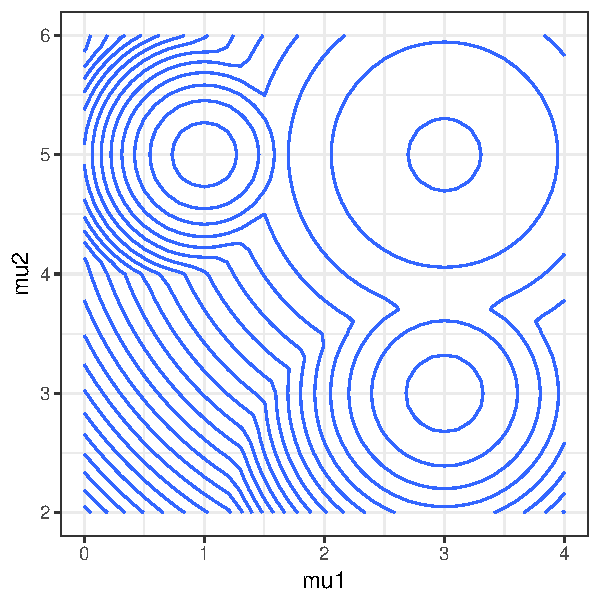
\includegraphics[width=1\textwidth]{fmm_mu_contour.pdf}
    \caption{Posterior density of the component means.}
    \end{subfigure}
    \end{center}
    \centering
   \begin{subfigure}[b]{0.32\textwidth}
    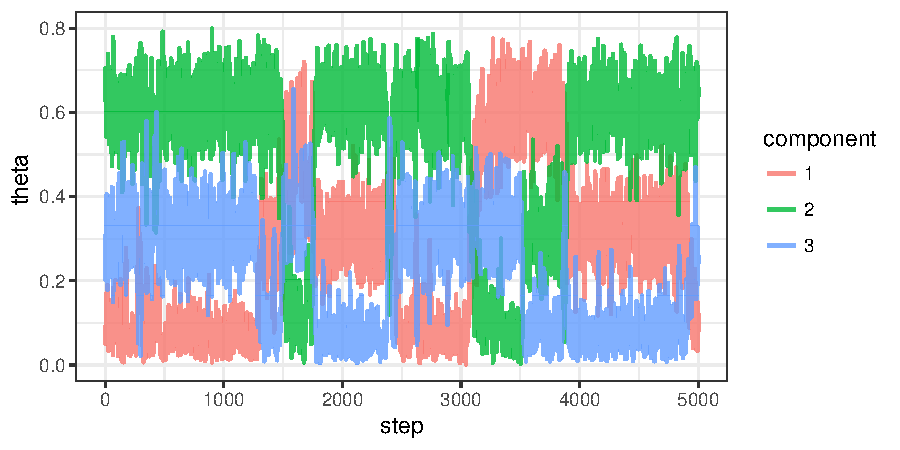
\includegraphics[width=1\textwidth]{fmm_w_gibbs.pdf}
    \caption{Gibbs sampling under canonical Dirichlet}
    \end{subfigure}
       \begin{subfigure}[b]{0.32\textwidth}
  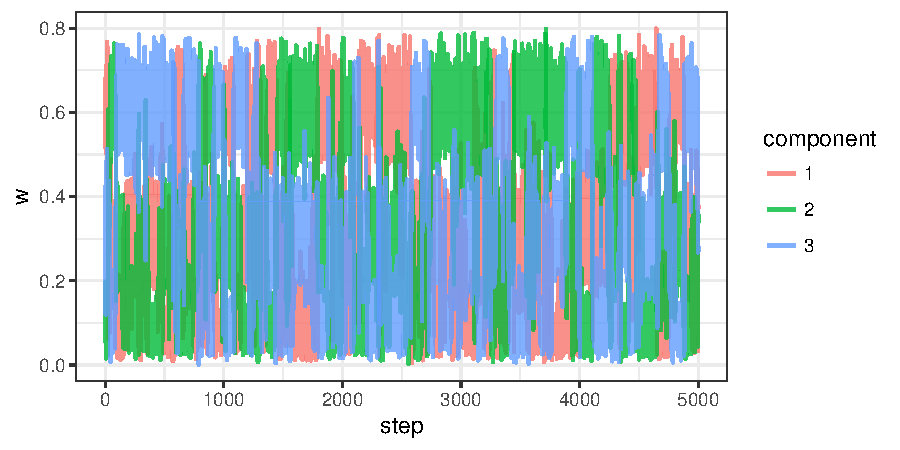
\includegraphics[width=1\textwidth]{fmm_w_hmc_unordered.pdf}
    \caption{HMC sampling under canonical Dirichlet, with extrinsic prior}
      \end{subfigure}
       \begin{subfigure}[b]{0.32\textwidth}
 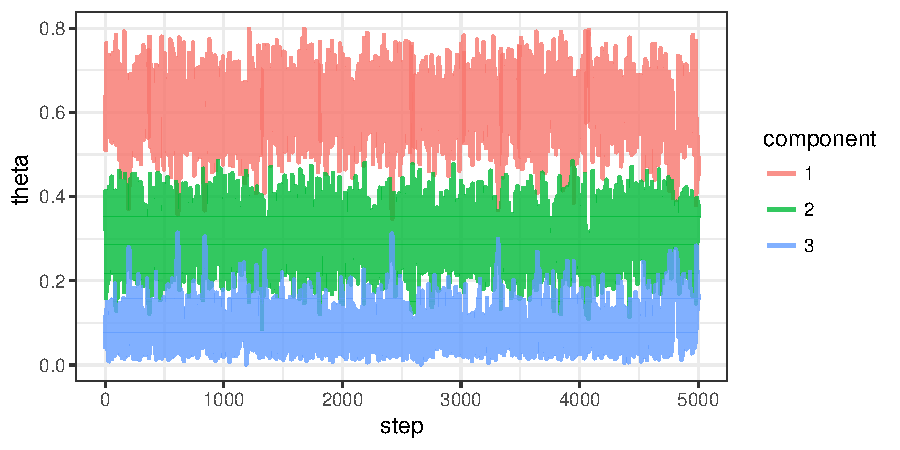
\includegraphics[width=1\textwidth]{fmm_w_hmc.pdf}
     \caption{HMC sampling under ordered Dirichlet, with extrinsic prior}
     \end{subfigure}
\caption{Contour of the posterior density of component means and traceplot of the posterior sample for the component weights $w$, in a 3-component normal mixture model. Panel (a) shows that there is significant overlap among component means $\mu_j$'s, creating label-switching issues in both Gibbs sampling (b) and HMC using canonical prior (c). The ordered Dirichlet prior significantly reducing label-switching (d).}
\label{dirichlet}
\end{figure}


{\bf Application 2: Orthonormal Tucker Factorization of Multiple Undirected Networks}

We now consider a real data application in brain network analysis. The brain connectivity structures are obtained in the data set KKI-42 (Landman et al. 2011), which consists of $21$ healthy subjects without any history of neurological disease. Each subject has two brain network observations from scan--rescan, yielding a total of n = 42. Each observation is a $V\times V$ symmetric network $A_i$, recorded as adjacency matrix $A_i$ for $i=1,\ldots,n$. For the $i$th matrix $A_i$, $A_{i,k,l} \in \{0,1\}$ is element on the $k$th row and $l$th column of $A_i$, with $A_{i,k,l}=1$ indicating there is an connection betwen $k$th and $l$th region, $A_{i,k,l}=0$ if there is no connection. The regions are constructed via the Desikan et al. (2006) atlas, for a total of V = 68 nodes.

The ambient dimension of observation is large $V(V-1)/2=2,278$ compared to sample size $n$, with potential observational error in recording connectivity. The diagonal in each $A_{i}$ is missing due to the lack of meaning in self-connectivity in brain network. These facts merit using a low-rank Bayesian approach.

% We first define an matrix operator that extracts its lower triangluar elements, for $V\times V$ matrix, $L(X)=\{X_{2,1}, X_{3,1}, \ldots X_{V,1}, X_{3,2}, X_{4,2}, \ldots X_{V,2},\ldots, X_{V,V-1}\}$. 

We consider a symmetric Bernoulli Tucker decomposition model:


 \begin{equation*}
\begin{aligned}
& A_{i,k,l} \sim \text{Bern}( \frac{1}{1+ \exp(-\psi_{i,k,l}- Z_{k,l})})\\
& \psi_{i,k,l} = \sum_{r_3=1}^{d1}\sum_{r_2=1}^{d1}\sum_{r_1=1}^{d3} D_{r_1,r_2,r_3} W_{i,r_1} U_{k,r_2} U_{l,r_3}  \\
\end{aligned}
\end{equation*}
for $k>l$, $k=2,\ldots, V$, $i=1,\ldots,n$; $U$ is $V\times d_1$ matrix, $W$ is $n\times d_2$ matrix. The symmetry of each network is induced by using $U$ twice in the decomposition. The core tensor $D$ is a $d_1\times d_1\times d_3$ array, whose entries correpond to the interaction between different factor; $D_{r_1,k,l}=D_{r_1,l,k}$ for all $r_1,k,l$. The  $V\times V$ matrix $Z$ is almost unstructural except symmetric $Z_{k,l}=Z_{l,k}$, which is commonly used to induce low-rank in the decomposition \citep{durante2016nonparametric}.

The Tucker decomposition is more flexible than another routinely used decomposition, namely parallel factor analysis (PARAFAC). The PARAFAC assumes all ranks are equal and the core tensor $D$ only has non-zero value when all its sub-indices are equal. In this case, PARAFAC would assume $d_1=d_3$ and $D_{r_1,r_2,r_3}=0$ unless $r_1=r_2=r_3$. The additional flexibility in the Tucker is appealing, as one would utilize the varying rank over different sub-direction (mode) of the tensor. On the other hand, a completely unconstrained Tucker decomposition is not identifiable in the matrices and core tensor, due to rotation and scaling. For example, one can multiply a $d_1\times d_1$ orthonormal matrix $R$, to $U$ and obtain $U^*=UR$ and each slice of $D_{r_1,.,}$ to obtain $D^*_{r_1,.,}=R'D_{r_1,.,}R$. This leaves the likelihood unchanged.

Therefore, we consider applying some constraint on the Tucker decomposition, while still maintaining its varying rank property over different modes. Motivated by high-order singular value decomposition, we first impose orthonormality constraints $U'U=I_{d_1}$ and $W'W=I_{d_3}$ and diagonal strucutre for all $D_{r_1,.,.}$, with $D_{r_1,r_2,r_3}=0$ unless $r_2=r_3$.
% We further force the first slice of the core $D_{1,.,.}$ to be diagonal, with $D_{1,r_2,r_3}=0$ unless $r_2=r_3$. This condition is set based on the observation that one can obtain a set of $U^*D^*_{r_i,.,.}U^{*'}$ for $r_i=1,\ldots,d_3$ and then rotate $P$ to make the first slice diagonal, where  $D^*_{1,.,.}=PD_{1,.,.}P'$. Fixing the first slice to diagonal remove such rotation without affecting flexibility.

We assign normal prior for $U_{k,r_2}\sim \No(0,\phi_{1})$, $W_{i,r_1}\sim \No(0,\phi_2)$, $Z_{k,l}\sim \No(0,\phi_3)$, $D_{r_1,r_2,r_2}\sim No(0, \phi_{4,r_1,r_2})$ for all $i,k,l,r_1,r_2$, and inverse-Gamma prior $\phi_1,\phi_2,\phi_3\stackrel{indep}{\sim} \text{IG}(2,1)$. For $\phi_{4,r_1,r_2}$, we assign multiplicative inverse gamma distribution \citep{bhattacharya2011sparse} $\phi_{4,r_1,r_2}= \prod_{m_1=1}^{r_1} \nu_{1,m_1} \prod_{m_2=1}^{r_2}  \nu_{2,m_2}$ with $\nu_{1,1},\nu_{2,1} \stackrel{indep}{\sim} \text{IG}(a_1,1)$ and $\nu_{1,m},\nu_{2,m}\stackrel{indep}{\sim} \text{IG}(a_2,1)$ for $m\ge 2$. This induces increasing concentration towards
zero as $r_1,r_2$ increase, allowing adaptive choosing of latent dimensions. We set $a_1=a_2=5$ in this application.

To allow estimation for model with orthonormality constraint, we use extrinsic prior with $\mc K(\theta) = \exp( - \frac{|U'U-I_{d_1}| + |W'W-I_{d_2}|  }{\lambda})$ and set $\lambda=10^{-3}$. To compare, we also test with the same model configuration without the orthonormality constraint, and refer to it as unconstrained model. We run both models for $10,000$ steps and discard the first $5,000$ steps. Figure~\ref{tucker} plots the traceplot and autocorrelation for matrix $U$. Unconstrained model has severe convergence issue due to the non-identifiability, while constrained model converges and show low autocorrelation for all the parameters.

\begin{figure}[H]
   \begin{subfigure}[b]{1\textwidth}
    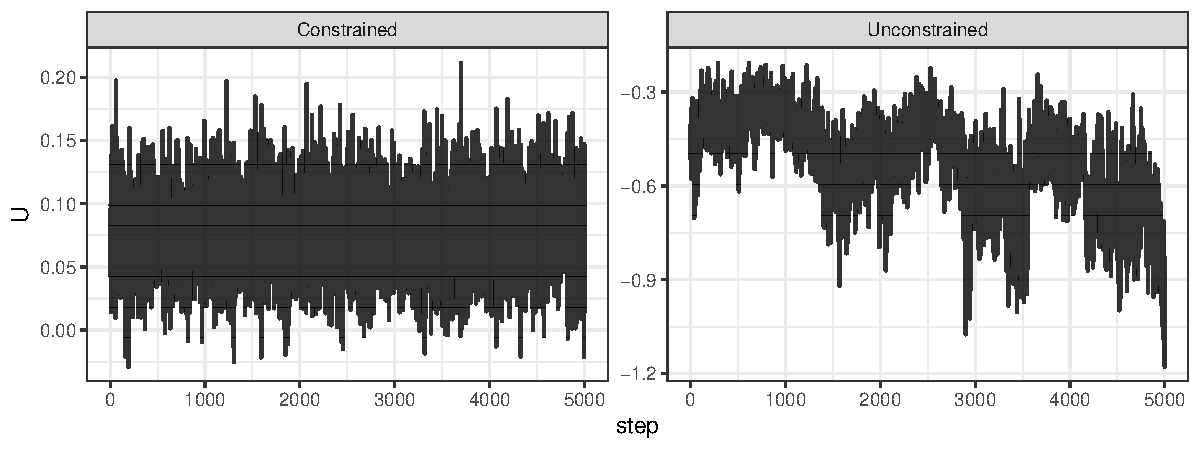
\includegraphics[width=1\textwidth]{tucker_traceplot.pdf}
    \caption{Traceplot of $U_{1,1}$.}
    \end{subfigure}
    \begin{subfigure}[b]{1\textwidth}
    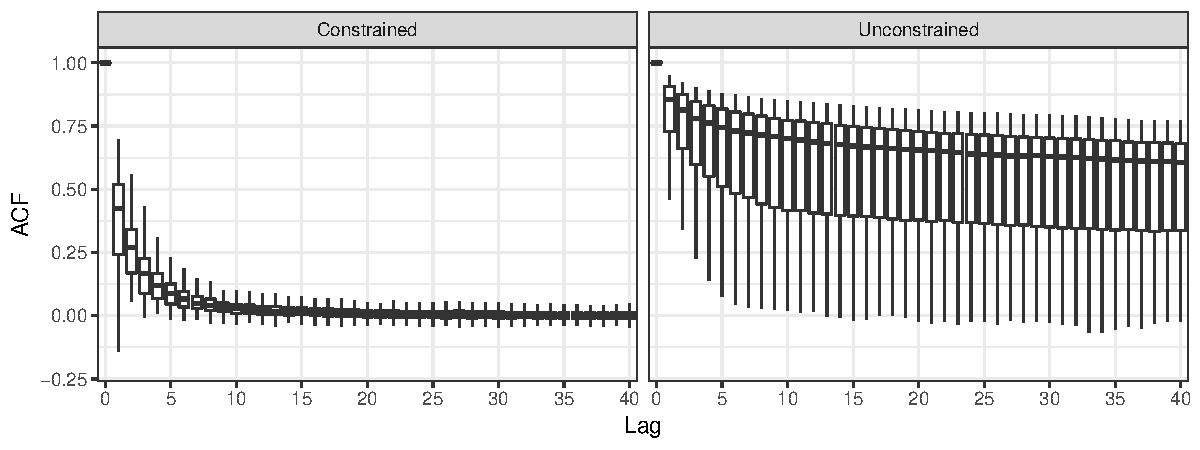
\includegraphics[width=1\textwidth]{tucker_acf.pdf}
    \caption{ACF of all elements in $U$}
    \end{subfigure}
\caption{Contour of the posterior density of component means and traceplot of the posterior sample for the component weights $w$, in a 3-component normal mixture model. Panel (a) shows that there is significant overlap among component means $\mu_j$'s, creating label-switching issues in both Gibbs sampling (b) and HMC using canonical prior (c). The ordered Dirichlet prior significantly reducing label-switching (d).}
\label{tucker}
\end{figure}

Ignoring those $D_{r_1,r_2,r_3}$ corresponding to $\phi_{4,r_1,r_2}<10^{-3}$, the multiplicative prior results in effective $\tilde{d}_1=5$ and $\tilde{d}_3=3$ dimensions.

\section{Discussion}



\bibliography{reference}
\bibliographystyle{chicago}

\end{document}



We now illustrate a curve fitting problem where the shape of curve is convex. Convexity is common in real life such as a trajectory of projectile or accelerated decreasing of organ functions in disase monitinoring. Consider a cubic spline function $f(t)$ for data $y_t$ with $t\in [0,1]$


\begin{equation*}
\begin{aligned}
y_t & = f(t) + \epsilon_t,\\
f(t) & = \beta_0 + \beta_1 t + \beta_2 t^2+ \beta_3 t^3+ \sum_{j=1}^J b_j (t- \tau_j)^3_+,\\
\end{aligned}
\end{equation*}
where $\epsilon_t \sim \No(0, \sigma^2)$ and $\tau_j$'s are pre-specified knots in $(0,1)$. To induce the convexity, it suffices to have the second derivative:

\begin{equation*}
\begin{aligned}
f''(t) & =  2\beta_2 + 6\beta_3 t+ \sum_{j=1}^J 6b_j (t- \tau_j)_+ \ge 0.\\
\end{aligned}
\end{equation*}

Given data $y_t$ at observed time $t=t_1,\ldots, t_n$, the posterior estimation of $\beta_.$ and $b_.$ is estimated under $n$ linear inequality constraints.

